% 2.0.SampleBuild.tex
%	Last update: 2021/03/02 F.Kanehori
\newpage
\section{サンプルプログラムのビルド}
\label{sec:SampleBuild}
\parindent=0pt

サンプルプログラムのビルド方法について説明します。
サンプルプログラムでは\SprLib を使用しますので、予めビルドしておいてください。

\bigskip
サンプルプログラムは、\SprTop{\core\src\Samples}以下に置かれています。
ここでは``BoxStack''を例にして説明します。

\bigskip
\SprTop{\core\src\Samples\Physics\BoxStack}に移動します。

適切なバージョンのソリューションファイル
\Path{BoxStack##.#.sln}をVisual Studioで開き、
プロジェクト\tt{BodStack}をスタートアッププロジェクトに設定してビルドすれば
実行形式バイナリが生成されます。

\begin{narrow}[15pt]
	\begin{figure}[h]
	\begin{center}
	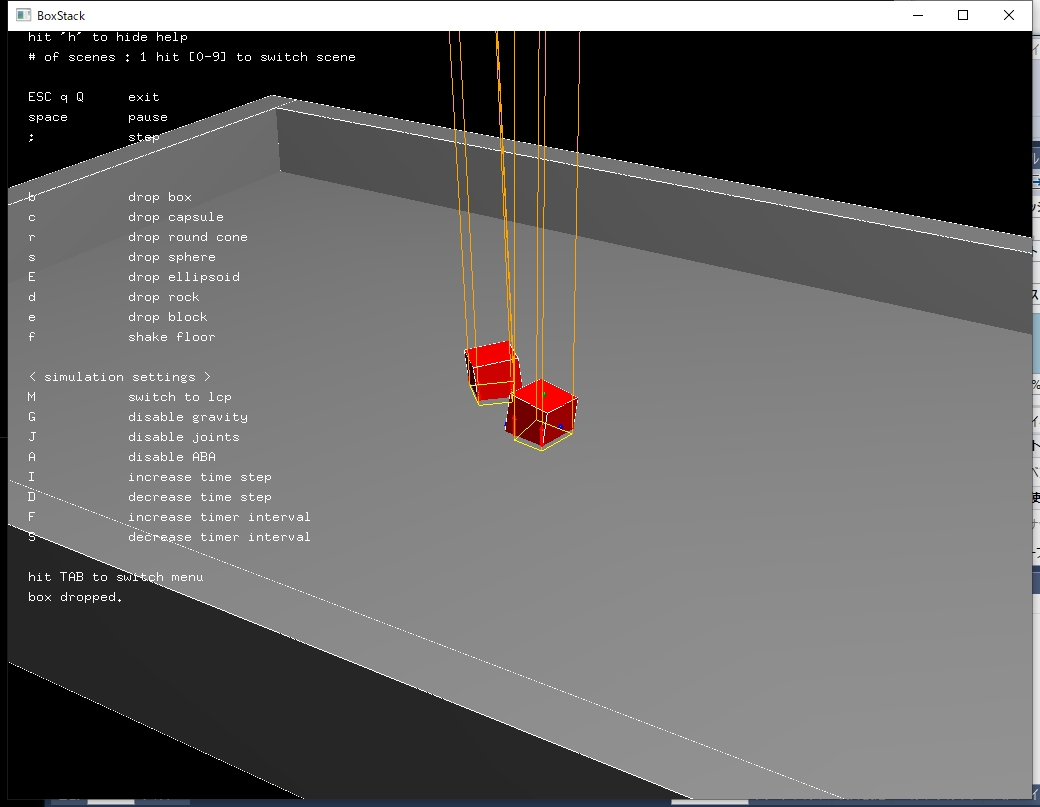
\includegraphics[width=0.5\textwidth]{fig/BoxStack_run.eps}
	\end{center}
	\caption{実行結果}
	\label{fig:BoxStack_run}
	\end{figure}
\end{narrow}


\bigskip
% end: 2.0.SampleBuild.tex
